%%&presentation-preformat

% --- Определение класса документа --- %

\newif\ifpresentation % Условие, проверяющее, что документ --- презентация
\presentationtrue
\documentclass[10pt, xcolor={dvipsnames, table, hyperref}]{beamer}

% --- Подключение общих новых переменных, данных и стилей --- %

% ------------------------------------------------------------------------------ %
% --- Файл упрощённых настроек шаблона, общих для диссертации и автореферата --- %
% ------------------------------------------------------------------------------ %

% --- Режим черновика --- %

\makeatletter
\@ifundefined{c@draft}{
	\newcounter{draft}
    \setcounter{draft}{0} % 0 -- чистовик (максимальное соблюдение ГОСТ)
                          % 1 -- черновик (отклонения от ГОСТ, но быстрая 
                          %       сборка итоговых PDF)
}{}
\makeatother

% --- Пометки в тексте --- %

\makeatletter
\@ifundefined{c@showmarkup}{
	\newcounter{showmarkup}
	\setcounter{showmarkup}{0} % 0 -- скрыть пометки
                               % 1 -- показывать пометки
}{}
\makeatother

% --- Использование в pdflatex шрифтов не по-умолчанию --- %

\makeatletter
\@ifundefined{c@usealtfont}{
  \newcounter{usealtfont}
  \setcounter{usealtfont}{2} % 0 -- шрифты на базе Computer Modern
                             % 2 -- использовать пакет XCharter, 
                             %       при наличии подходящей версии
}{}
\makeatother

% --- Вывод типов ссылок в библиографии --- %

\makeatletter
\@ifundefined{c@mediadisplay}{
	\newcounter{mediadisplay}
    \setcounter{mediadisplay}{1} % 0 -- не делать ничего; надписи [Текст] и
                                 %       [Эл. ресурс] будут выводиться только в ссылках с
                                 %       заполненным полем `media`;
                                 % 1 -- автоматически добавлять надпись [Текст] к ссылкам с
                                 %       незаполненным полем `media`; таким образом, у всех
                                 %       источников будет указан тип, что соответствует
                                 %       требованиям ГОСТ
                                 % 2 -- автоматически удалять надписи [Текст], [Эл. Ресурс] и др.;
                                 %       не соответствует ГОСТ
                                 % 3 -- автоматически удалять надпись [Текст];
                                 %       не соответствует ГОСТ
                                 % 4 -- автоматически удалять надпись [Эл. Ресурс];
                                 %       не соответствует ГОСТ
}{}
\makeatother

% --- Предкомпиляция tikz рисунков для ускорения работы --- %

\makeatletter
\@ifundefined{c@imgprecompile}{
	\newcounter{imgprecompile}
	\setcounter{imgprecompile}{0} % 0 -- без предкомпиляции;
                                  % 1 -- пользоваться предварительно
                                  %       скомпилированными pdf вместо генерации
                                  %       заново из tikz
}{}
\makeatother
    % Общие настройки шаблона
% ---------------------------------------------------------------------- %
% --- Пакеты, которые являются общими для диссертации и автореферата --- %
% ---------------------------------------------------------------------- %

% --- Логические условия --- %

\newif\ifsynopsis     % Условие, проверяющее, что документ является авторефератом
\usepackage{etoolbox}
\providebool{presentation}

% --- Комментирование текста --- %

\usepackage{comment}    

% --- Поля и разметка страницы --- %

\usepackage{pdflscape} % Для включения альбомных страниц
\usepackage{geometry}  % Для последующего задания полей

% --- Математические пакеты --- %

\usepackage{amsthm, amsmath, amscd} % Математические дополнения от AMS
\usepackage{amsfonts, amssymb}      % Математические дополнения от AMS
\usepackage{mathtools}              % Добавляет окружение multlined
\usepackage{xfrac}                  % Красивые дроби
\usepackage{upgreek}                % Русская традиция начертания греческих букв

% --- Кодировки и шрифты --- %

% Кириллица в нумерации subequations
\patchcmd{\subequations}{\def\theequation{\theparentequation\alph{equation}}}
{\def\theequation{\theparentequation\asbuk{equation}}}
{\typeout{subequations patched}}{\typeout{subequations not patched}}

% Установки для размера шрифта 14 pt
\newlength{\curtextsize}
\newlength{\bigtextsize}
\setlength{\bigtextsize}{13.9pt}
\makeatletter
\setlength{\curtextsize}{\f@size pt}
\makeatother

% Решение проблемы копирования текста в буфер кракозябрами
\ifnumequal{\value{usealtfont}}{0}{}{
    \input glyphtounicode.tex
    \input glyphtounicode-cmr.tex %from pdfx package
    \pdfgentounicode=1
}
    
% Улучшенный поиск русских слов в полученном pdf-файле
\usepackage{cmap}   
\ifnumequal{\value{usealtfont}}{2}{}{
    \defaulthyphenchar=127  % Если стоит до fontenc, то переносы
                            % не впишутся в выделяемый текст при
                            % копировании его в буфер обмена
}

% Дополнительные текстовые символы
\usepackage{textcomp}

% Языковые пакеты
\usepackage[T1, T2A]{fontenc}        % Поддержка русских букв
\usepackage[utf8]{inputenc}          % Кодировка utf8
\usepackage[english, russian]{babel} % Языки: русский, английский

% Подключение русифицированных шрифтов XCharter
\ifnumequal{\value{usealtfont}}{2}{
	\usepackage[scaled = 0.914]{XCharter} 
	%\usepackage[charter, vvarbb, scaled = 1.048]{newtxmath}
	\ifpresentation
	\else
		\setDisplayskipStretch{-0.078}
	\fi
}{}

% --- Оформление абзацев --- %

% Красная строка после заголовков типа chapter
\ifpresentation
\else
    \indentafterchapter
    \usepackage{indentfirst}
\fi

% --- Цвета --- %

\ifpresentation
\else
    \usepackage[dvipsnames, table, hyperref]{xcolor}
\fi

% --- Таблицы --- %

\usepackage{threeparttable} % Автоматическая ширина подписи таблицы
\usepackage{tabularray}     % Таблицы с гибкими настройками

% --- Общее форматирование --- %

\usepackage{soulutf8} % Поддержка переносоустойчивых подчёркиваний и зачёркиваний

% --- Оптимизация расстановки переносов и длины последней строки абзаца --- %

\usepackage[hyphenation, lastparline]{impnattypo}

% --- Работа со списками --- %

\ifpresentation
\else
	\usepackage{enumitem}
\fi

% --- Векторная графика --- %

\usepackage{stanli}   % Отрисовка конструкций
\usepackage{tikz}     % Пакет векторной изображений 
\usepackage{pgfplots} % Построение векторных графиков

% Пакеты Tikz
\usetikzlibrary{shadows}     				% Тени
\usetikzlibrary{arrows.meta} 				% Стрелки
\usetikzlibrary{positioning} 				% Позиционирование 
\usetikzlibrary{calc}        				% Расчетная библиотека
\usetikzlibrary{trees} 		 				% Построение деревьев
\usetikzlibrary{external}	 				% Компиляция изображений
\usetikzlibrary{decorations.pathreplacing}  % Изменения отображения пути
\usetikzlibrary{calligraphy}  				% Каллиграфия
\usetikzlibrary{angles}						% Отображение углов
\usetikzlibrary{patterns}					% Штриховка

% --- Гиперссылки --- %

\usepackage{color}
\usepackage{hyperref}

% --- Изображения --- %

\usepackage{graphicx}   % Подключаем пакет работы с графикой
\usepackage{caption}    % Подписи рисунков и таблиц
\usepackage{subcaption} % Подписи подрисунков и подтаблиц
\usepackage{pdfpages}   % Добавление внешних pdf файлов
\usepackage{float}      % Дополнительные опции размещения

% --- Счётчики --- %

\usepackage{aliascnt}                  % Псевдонимы счетчиков
\usepackage[figure, table]{totalcount} % Счётчик рисунков и таблиц
\usepackage{totcount}                  % Пакет создания счётчиков на основе последнего номера
                                       %  подсчитываемого элемента (может требовать дважды
                                       %  компилировать документ)
\usepackage{totpages}                  % Счётчик страниц, совместимый с hyperref (ссылается
                                       %  на номер последней страницы). Желательно ставить
                                       %  последним пакетом в преамбуле

% --- Управление групповыми ссылками --- %

\ifpresentation
\else
	\usepackage[russian]{cleveref}
\fi

% --- При работе с черновиком --- %

\ifnumequal{\value{draft}}{1}{
    \usepackage[firstpage]{draftwatermark}
    \SetWatermarkText{DRAFT}
    \SetWatermarkFontSize{14pt}
    \SetWatermarkScale{15}
    \SetWatermarkAngle{45}
}{} % Пакеты общие для диссертации и автореферата
% --------------------------------------- %
% --- Основные сведения о диссертации --- %
% --------------------------------------- %

% --- Данные автора --- %

\newcommand{\thesisAuthorLastName}{Лакиза}
\newcommand{\thesisAuthorOtherNames}{Павел Анатольевич}
\newcommand{\thesisAuthorInitials}{П.\,А.}
\newcommand{\thesisAuthor}             
{%
	\texorpdfstring{
        \thesisAuthorLastName~\thesisAuthorOtherNames  % Так будет отображаться на титульном листе или в тексте, где будет использоваться переменная
    }{%
        \thesisAuthorLastName, \thesisAuthorOtherNames % Эта запись для свойств pdf-файла. В таком виде, если pdf будет обработан программами для сбора библиографических сведений, будет правильно представлена фамилия.
    }
}
\newcommand{\thesisAuthorShort}{\thesisAuthorInitials~\thesisAuthorLastName}

% --- Данные диссертации --- %

\newcommand{\thesisTitle}{Коррекция расчетных моделей летательных аппаратов по результатам модальных испытаний}
\newcommand{\thesisTitleShort}{Коррекция расчетных моделей ЛА по результатам модальных испытаний}
\newcommand{\thesisSpecialtyNumber}{2.5.14}
\newcommand{\thesisSpecialtyTitle}{Прочность и тепловые режимы летательных аппаратов}
\newcommand{\thesisDegree}{кандидата технических наук}
\newcommand{\thesisDegreeShort}{канд.~тех.~наук}
\newcommand{\thesisCity}{Новосибирск}
\newcommand{\thesisYear}{2023}

% --- Данные первой организации --- %

\newcommand{\thesisFirstOrganization}{Федеральное автономное учреждение <<Сибирский научно-исследовательский институт авиации им.~С.\,А.~Чаплыгина>>}
\newcommand{\thesisInFirstOrganization}{Федеральном автономном учреждении <<Сибирский научно-исследовательский институт авиации им.~С.\,А.~Чаплыгина>>}
\newcommand{\thesisFirstOrganizationShort}{СибНИА~им.~С.\,А.~Чаплыгина}

% --- Данные второй организации --- %

\newcommand{\thesisSecondOrganization}{Федеральное государственное бюджетное образовательное учреждение высшего образования <<Новосибирский государственный технический университет>>}
\newcommand{\thesisInSecondOrganization}{Федеральном государственном бюджетном образовательном учреждении высшего образования <<Новосибирский государственный технический университет>>}
\newcommand{\thesisSecondOrganizationShort}{НГТУ}

% --- Данные научного руководителя --- %

\newcommand{\supervisorFio}{Бернс Владимир Андреевич}
\newcommand{\supervisorRegalia}{доктор технических наук,~профессор}
\newcommand{\supervisorFioShort}{В.\,А.~Бернс}
\newcommand{\supervisorRegaliaShort}{д-р техн.~наук,~проф.}

% --- Данные первого оппонента --- %

\newcommand{\opponentOneFio}{Щеглов Георгий Александрович}
\newcommand{\opponentOneRegalia}{доктор технических наук, профессор}
\newcommand{\opponentOneJobPlace}{Федеральное государственное бюджетное образовательное учреждение
высшего образования <<Московский государственный технический университет имени Н.\,Э.~Баумана (национальный исследовательский университет)>>}
\newcommand{\opponentOneJobPost}{кафедра <<Аэрокосмические системы>>, профессор}

% --- Данные второго оппонента --- %

\newcommand{\opponentTwoFio}{Иголкин Александр Алексеевич}
\newcommand{\opponentTwoRegalia}{доктор технических наук, доцент}
\newcommand{\opponentTwoJobPlace}{Федеральное государственное автономное образовательное учреждение высшего образования <<Самарский национальный исследовательский университет имени академика С.\,П.~Королева>>}
\newcommand{\opponentTwoJobPost}{кафедра <<Автоматические системы энергетических установок>>, профессор}

% --- Данные о ведущей организации --- %

\newcommand{\leadingOrganizationTitle}{Федеральное автономное учреждение <<Центральный аэрогидродинамический институт имени профессора Н.\,Е.~Жуковского>>, г.~Жуковский}

% --- Данные о защите --- %

\newcommand{\defenseDate}{15 июня 2023~года~в~$ \text{14}\mspace{1mu} ^ \text{\underline{00}} $ часов}

% --- Данные диссертационного совета --- %

\newcommand{\defenseCouncilNumber}{24.2.347.03}
\newcommand{\defenseCouncilTitle}{Федерального государственного бюджетного образовательного учреждения высшего образования <<Новосибирский государственный технический университет>>}
\newcommand{\defenseCouncilAddress}{630073, г.~Новосибирск, проспект~К.~Маркса, 20, I корпус, конференц-зал}
\newcommand{\defenseCouncilPhone}{+7~(383)~346-06-12}
\newcommand{\defenseSecretaryFio}{Тюрин Андрей Геннадиевич}
\newcommand{\defenseSecretaryRegalia}{канд.~техн.~наук, доцент}

% --- Данные автореферата --- %

\newcommand{\synopsisSource}{в библиотеке Новосибирского государственного технического университета, а также на официальном сайте: \\ \href{https://www.nstu.ru/science/dissertation_sov/dissertations/view?id=19641}{\nolinkurl{www.nstu.ru/science/dissertation_sov/dissertations/view?id=19641}}}
\newcommand{\synopsisDate}{<<\underline{\hspace{2em}}>> апреля 2023~года}

% --- Ключевые слова для метаданных PDF диссертации и автореферата --- %

\providecommand{\keywords}{Летательный аппарат, коррекция расчетной динамической модели, конечно-элементная модель, экспериментальный модальный анализ, собственные колебания, обобщенные модальные характеристики, диагностирование дефектов, аэроупругая устойчивость}
     % Основные сведения

% --- Подключение специальных настроек шаблона и пакетов --- %

% ---------------------------------------------------------------------- %
% --- Пакеты, использующиеся только в презентации  --------------------- %
% ---------------------------------------------------------------------- %

% --- Математические пакеты --- %

\usepackage{mathtext} % Текст в математическом режиме
\usepackage{array}	  % Массивы
\usepackage{nicefrac} % Красивые дроби

% --- Разметка --- %

\usepackage{ragged2e} % Выравнивание плавающих объектов

% --- Списки --- %

\usepackage{enumerate} % Нумерованные списки

% --- Таблицы --- %

\usepackage{booktabs} % Закладки

% --- Приложения --- %

\usepackage{appendixnumberbeamer} % Не считать номера страниц после команды \appendix % Пакеты для презентации
% ----------------------------- %
% --- Стили для презентации --- %
% ----------------------------- %

% --- Шаблон --- %

\DeclareRobustCommand{\fixme}{\textcolor{red}}

% --- Путь к изображениям --- %

\graphicspath{{images/partReview/}{images/partModalAnalysis/}{images/partModelUpdating/}{images/partAprobation/}{images/appendix/}}

% --- Тема оформления --- %

\usetheme{Pittsburgh}
\usecolortheme{whale}

% --- Макет страниц --- %

\setbeamersize{text margin left = 1cm, text margin right = 1cm} % Размер полей слайдов

% --- Настройки навигации --- %

\beamertemplatenavigationsymbolsempty % Отключение стрелок

% --- Параметры шрифтов --- %

% Размеры шрифтов
\setbeamerfont{institute}{size = \small}
\setbeamerfont{author}{size = \large}
\setbeamerfont{title}{size = \large}
\setbeamerfont{subtitle}{size = \normalsize}
\setbeamerfont{date}{size = \normalsize}
\setbeamerfont{bibliography item}{size = \small}
\setbeamerfont{bibliography entry author}{size = \small}
\setbeamerfont{bibliography entry title}{size = \small}
\setbeamerfont{bibliography entry location}{size = \small}
\setbeamerfont{bibliography entry note}{size = \small}

% Шрифты с засечками для формул
\usefonttheme[onlymath]{serif} 

% --- Цвета структурных элементов --- %

\setbeamercolor{footline}{fg = blue}
\setbeamercolor{bibliography item}{fg = black}
\setbeamercolor{bibliography entry author}{fg = black}
\setbeamercolor{bibliography entry title}{fg = black}
\setbeamercolor{bibliography entry location}{fg = black}
\setbeamercolor{bibliography entry note}{fg = black}

% --- Настройки библиографии --- % 

\setbeamertemplate{bibliography item}{\insertbiblabel} % Нумерация списка статей

% --- Настройки гиперссылок --- %

\hypersetup{
    unicode = true, % Не латинские символы в закладках
}

% --- Настройка списков --- %

\makeatletter
\newcommand*{\rom}[1]{\expandafter\@slowromancap\romannumeral#1@}
\makeatother

\newcommand{\itemi}{\item[\checkmark]}

% --- Разметка нижнего колонтитула --- %

\setbeamertemplate{footline}{
    \leavevmode%
    \hbox{%
    	% Автор 
        \begin{beamercolorbox}[wd=.333333\paperwidth,ht=2.25ex,dp=1ex,center]{}%
            \thesisAuthorShort, \thesisFirstOrganizationShort
        \end{beamercolorbox}%
        % Город
        \begin{beamercolorbox}[wd=.333333\paperwidth,ht=2.25ex,dp=1ex,center]{}%
            \thesisCity, \thesisYear
        \end{beamercolorbox}%
        % Страницы
        \begin{beamercolorbox}[wd=.333333\paperwidth,ht=2.25ex,dp=1ex,right]{}%
            Стр. \insertframenumber{} из \inserttotalframenumber \hspace*{2ex}
        \end{beamercolorbox}}%
    \vskip0pt%
}	  % Стили презентации
% ---------------------- %
% --- Титульный лист --- %
% ---------------------- %

% Шаблон оформления титульной страницы
\setbeamertemplate{title page}
{
	% Названия организаций
	\centering
	\usebeamerfont{institute}
	Федеральное автономное учреждение <<Сибирский научно-исследовательский \\ институт авиации им.~С.\,А.~Чаплыгина>> \\
	Федеральное государственное бюджетное образовательное учреждение высшего образования <<Новосибирский государственный технический университет>> \\
	\par
	\rule{\linewidth}{0.5pt}
	% Данные автора
	\centering
	\vfill
	\usebeamerfont{author}\insertauthor\par
	% Название работы
	\vfill
	\begin{beamercolorbox}[sep=8pt, center]{title}
		\usebeamerfont{title}
		Коррекция расчетных моделей летательных аппаратов \\ по результатам модальных испытаний
		\par%
    \end{beamercolorbox}%
	% Данные о специальности
	\vfill
	\usebeamerfont{subtitle}
	Специальность 2.5.14 --- Прочность и тепловые режимы летательных \\ \hspace{-4.5em} аппаратов	
	\par
	% Данные о научном руководителе
	\vfill
	\begin{flushright}
		Научный руководитель: \\
		\supervisorRegalia \\
		\supervisorFio
	\end{flushright}
	% Дата
    \vfill
    \usebeamerfont{date}\insertdate\par
    {\usebeamercolor[fg]{titlegraphic}\inserttitlegraphic\par}
}

% Данные полей шаблона
\institute{\thesisFirstOrganization\newline\thesisSecondOrganization}
\author{\thesisAuthor}
\title{\thesisTitle}
\subtitle{Специальность \thesisSpecialtyNumber~---~\thesisSpecialtyTitle}
\date{\thesisCity, \thesisYear}	  % Настройки заглавной страницы

% --- Подключение библиографии --- %

% --------------------------------------------------------- %
% --- Настройки библиографии посредством движка bibtex8 --- %
% --------------------------------------------------------- %

% --- Пакеты --- %

\usepackage{cite} % Ссылки на литературу

% --- Стили --- %

% Оформляем библиографию по ГОСТ 7.1 (ГОСТ Р 7.0.11-2011, 5.6.7)
\bibliographystyle{biblio/ugost2008cust} 

% Заменяем библиографию с квадратных скобок на точку
\makeatletter
\renewcommand{\@biblabel}[1]{#1.}   
\makeatother

% --- Цитирование --- %

% Разделение ; при перечислении ссылок (ГОСТ Р 7.0.5-2008)
\renewcommand\citepunct{;\penalty\citepunctpenalty\hskip.13emplus.1emminus.1em\relax} 

% Чтобы примеры цитирования, рассчитанные на biblatex, не вызывали ошибок при компиляции в bibtex
\newcommand*{\autocite}[1]{}  

% --- Создание команд для вывода списка литературы --- %

\newcommand*{\insertbibliofull}{\bibliography{biblio/external, biblio/author}}
\newcommand*{\insertbiblioauthor}{\bibliography{biblio/author}}
\newcommand*{\insertbiblioexternal}{\bibliography{biblio/external}}

% Счётчик использованных ссылок на литературу, обрабатывающий с учётом неоднократных ссылок
\newtotcounter{citenum}
\def\oldcite{}
\let\oldcite=\bibcite
\def\bibcite{\stepcounter{citenum}\oldcite}


% --- Метка окончания предкомпиляции --- %

\csname endofdump\endcsname

% --- Вывод отладочной информации --- %

\listfiles

% --- Формирование документа --- %

\begin{document}
	% Преамбула презентации
	
% Титульный слайд
\begin{frame}[noframenumbering, plain]
    \setcounter{framenumber}{1}
    \maketitle
\end{frame}

\section{Введение}

\begin{frame}{Постановка задачи}
	\textbf{\underline{Цель диссертационной работы}}: разработка методики коррекции расчетных моделей летательных аппаратов по результатам модальных испытаний.
	\begin{center}
		\includegraphics[width = 0.8\textwidth]{example-airplane}
	\end{center}
\end{frame}

\begin{frame}{Задачи исследования}
	\begin{enumerate}
		\item Разработать методику коррекции расчетных динамических моделей ЛА по экспериментально определенным модальным характеристикам.
		\item Изучить методы классического модального анализа. Создать комплекс программ для обработки и представления результатов модального анализа непосредственно в процессе испытаний.
		\item Изучить методы операционного модального анализа. Разработать программное обеспечение для определения модальных характеристик ЛА по результатам акустических и летных испытаний.
		\item Изучить методы вибродиагностики конструкций. Разработать программное обеспечение для контроля конструктивно-производственных дефектов в конструкциях ЛА в процессе модальных испытаний.
		\item Оценить сходимость и чувствительность методики коррекции к погрешностям в результатах модальных испытаний.
		\item Решить практические задачи коррекции расчетных моделей конструкций.
	\end{enumerate}
\end{frame}

\begin{frame}{Положения, выносимые на защиту}
	\begin{enumerate}
		\item Методика коррекции расчетных динамических моделей путем добавления корректирующих конечных элементов, параметры которых определяются из решения задачи оптимизации по целевым модальным характеристикам.
		\item Методика синтеза расчетной модели ЛА из полноразмерных моделей составных частей, скорректированных по результатам модальных испытаний.
		\item Комплекс программ для обработки и представления результатов экспериментального модального анализа. Программное обеспечение коррекции и синтеза расчетных моделей ЛА.
		\item Результаты исследования сходимости алгоритма и чувствительности методики коррекции расчетных моделей к погрешностям эксперимента.
		\item Результаты решения практических задач.
	\end{enumerate}
\end{frame}

\begin{frame}{Обзор публикаций по теме исследования}
	\begin{itemize}
		\item \textbf{Стохастические методы коррекции}: \\ Beck~J.\,L., Katafygiotis~L.\,S., Boulkaibet~I., Vanik~M.\,W., Goller~B., Schueller~G.\,I., Au~S.\,K., Marwala~T., Yuen~K.\,V., Worden~K., Hensman~J.\,J., Cheung~S.\,H., Mthembu~L., Yan~W.\,J.
		\item \textbf{Детерминированные методы коррекции}: \\ Bakir~P.\,G., Friswell~M.\,I., Baruch~M., Mottershead~J.\,E., Ewins~D.\,J., Berman~E.\,G., Allen~M.\,S., Link~M., Park~D.\,C., Caesar~B., Min~C.\,H., Sipple~J.\,D., Gupta~A.
		\item \textbf{Методы регуляризации}: \\ Ahmadian~H., Fregolent~A., Natke~H.\,G., Visser~W.\,J., Titurus~B., Imregun~M., D'Ambrogio~W., Gladwell~G.\,M.\,L., Ismail~F., Hansen~P.\,C., Bartilson~D.\,T., Smyth~A.\,W.
		\item \textbf{Теоретические и практические аспекты методов модальных испытаний}: \\ Резник~А.\,Л., Смыслов~В.\,И., Микишев~Г.\,Н., Рабинович~Б.\,И., Бернс~В.\,А., Dat~R., Clerc~D., Kennedy~C.\,C., Pancu~C.\,D.\,P., Heylen~W., Lammens~S., Sas~P.
	\end{itemize}
\end{frame}   
	
	% Основное содержание
	\section{Методика коррекции конечно-элементных моделей ЛА}

\begin{frame}{Принципиальная схема коррекции}
	\begin{center}
		\begin{tikzpicture}[scale = 1]
			\pgfmathsetmacro{\nodeDist}{0.1}
			\pgfmathsetmacro{\shiftText}{0.0}
			% Исходная модель
			\node[inner sep = 0pt] (initial) at (0, 0) {\includegraphics[width = 0.3\textwidth]{simple-model-initial}};
			\node[inner sep = 0pt, below = \shiftText of initial.south] (textInitial) {Исходная модель};
			% Знак
			\node [font = \fontsize{30}{32}, below = \nodeDist of textInitial.south, color = blue] (sumSign) {\bfseries +};
			% Коррректирующие элементы
			\node[inner sep = 0pt, below = -\nodeDist of sumSign.south] (elements) {\includegraphics[width = 0.3\textwidth]{simple-model-elements}};
			\node[inner sep = 0pt, below = \shiftText of elements.south] (textElements) {Корректирующие элементы};
			% Скорректированная модель
			\draw (sumSign.east) ++ (2.25, 0) node [right] (updated) {\includegraphics[width = 0.5\textwidth]{simple-model-updated}};
			\draw [line width = 0.75mm, -{Latex[length = 6mm]}, color = red](sumSign.east) ++ (1.25, 0) --++ (1.75, 0);
			\node[inner sep = 0pt, below = \shiftText of updated.south] (textUpdated) {Скорректированная модель};
		\end{tikzpicture}
	\end{center}
\end{frame}

\begin{frame}{Методика коррекции конечно-элементной модели}
	\begin{block}{Обобщенная проблема собственных значений}
		\begin{equation}
			(\mat{K} - \lambda \mat{M}) \mat{Y} = 0,
		\end{equation}
		где $ \mat{K} $, $ \mat{M} \in \set{R} ^ {n \times n}$~---~матрицы жесткости и масс; $ \mat{Y} $~---~формы собственных колебаний; $ \lambda $~---~собственные числа; $ N $~---~число степеней свободы.
	\end{block}
	\begin{block}{Корректирующая матрица жесткости в общем виде}
 		\begin{equation}
 			\begin{gathered}
 				\Delta \mat{K} = \Delta \internal{\mat{K}} + \Delta \external{\mat{K}}, \\
				\Delta \internal{\mat{K}}_j = \sum\limits_{p\,=\,1}^{q} \internal{c}_{j+p-1} \mat{G}_j^{(p)}, \ j = 1 \hdots e, \\
				\Delta \external{\mat{K}} = \operatorname{diag} \cbrackets{\external{c}_1, \external{c}_2, \hdots, \external{c}_N}.
			\end{gathered}
		\end{equation}
		где $ \internal{\mat{c}} $ и $ \external{\mat{c}} $~---~неизвестные внутренние и внешние корректирующие жесткости; $ \mat{G}_j^{(p)} $~---~матрица внутреннего коррректирующего элемента, составленная из длин и направляющих косинусов; $ q $~---~число корректирующих жесткостей, описывающих элемент; $ e $~---~число внутренних корректирующих элементов.
	\end{block}
\end{frame}

\begin{frame}{Внутренний корректирующий элемент в виде балки}
	\begin{block}{Матрицы корректирующего элемента}
		\begin{equation*}
		\begingroup
		\setlength\arraycolsep{2pt}
		\begin{gathered}
			\mat{G}_j^{(1)} =
			\begin{pmatrix}
				\mat{D}_1 & \mat{0} & -\mat{D}_1 & \mat{0} \\
				\mat{0} & \mat{0} & \mat{0} & \mat{0} \\
				-\mat{D}_1 & \mat{0} & \mat{D}_1 & \mat{0} \\
				\mat{0} & \mat{0} & \mat{0} & \mat{0} \\
			\end{pmatrix},
			\mat{G}_j^{(2)} =
			\begin{pmatrix}
				6 \mat{D}_2 & 3 \ell \mat{D}_4 & -6 \mat{D}_2 & 3 \ell \mat{D}_4 \\
				3 \ell \trans{\mat{D}}_4 & 2 \ell ^ 2 \mat{D}_3 & -3 \ell \trans{\mat{D}}_4 & \ell ^ 2 \mat{D}_3 \\
				-6 \trans{\mat{D}}_2 & -3 \ell \mat{D}_4 & 6 \mat{D}_2 & -3 \ell \mat{D}_4 \\
				3 \ell \trans{\mat{D}}_4 & \ell ^ 2 \trans{\mat{D}}_3 & -3 \ell \trans{\mat{D}}_4 & 2 \ell ^ 2 	\mat{D}_3
			\end{pmatrix}, \\
			\mat{G}_j^{(3)} =
			\begin{pmatrix}
				6 \mat{D}_3 & -3 \ell \trans{\mat{D}}_4 & -6 \mat{D}_3 & -3 \ell \trans{\mat{D}}_4 \\
				-3 \ell \mat{D}_4 & 2 \ell ^ 2 \mat{D}_2 & 3 \ell \mat{D}_4 & \ell ^ 2 \mat{D}_2 \\
				-6 \trans{\mat{D}}_3 & 3 \ell \trans{\mat{D}}_4 & 6 \mat{D}_3 & 3 \ell \trans{\mat{D}}_4 \\
				-3 \ell \mat{D}_4 & \ell ^ 2 \trans{\mat{D}}_2 & 3 \ell \mat{D}_4 & 2 \ell ^ 2 \mat{D}_2
			\end{pmatrix},
			\mat{G}_j^{(4)} =
			\begin{pmatrix}
				\mat{0} & \mat{0} & \mat{0} & \mat{0} \\
				\mat{0} & \mat{D}_1 & 0 & -\mat{D}_1 \\
				\mat{0} & \mat{0} & \mat{0} & \mat{0} \\
				\mat{0} & -\mat{D}_1 & 0 & \mat{D}_1 \\
			\end{pmatrix},
		\end{gathered}
		\endgroup
		\end{equation*}
	\end{block}
	\begin{block}{Матрицы из направляющих косинусов}
		\begin{equation*}
			\mat{D}_k = 
			\begin{pmatrix}
				d_{k, 1}^2 & d_{k, 1} d_{k, 2} & d_{k, 1} d_{k, 3} \\
				d_{k, 2} d_{k, 1} & d_{k, 2} ^ 2 & d_{k, 2} d_{k, 3} \\
				d_{k, 3} d_{k, 1} & d_{k, 3} d_{k, 2} & d_{k, 3} ^ 2
				\end{pmatrix},
			\mat{D}_4 = 
			\begin{pmatrix}
				d_{2, 1} d_{3, 1} & d_{2, 1} d_{3, 2} & d_{2, 1} d_{3, 3} \\
				d_{2, 2} d_{3, 1} & d_{2, 2} d_{3, 2} & d_{2, 2} d_{3, 3} \\
				d_{2, 3} d_{3, 1} & d_{2, 3} d_{3, 2} & d_{2, 3} d_{3, 3}
			\end{pmatrix},
		\end{equation*}
	\end{block}
	где $ \ell $~---~длина корректирующего балочного элемента, $ k = 1 \hdots 3 $.
\end{frame}

\begin{frame}{Расчет корректирующих жесткостей}
	\begin{block}{Задача безусловной минимизации}
		\vspace{-1em}
		\begin{gather}
			f_j(c) = \mat{Y}_j^{(0)\mathsf{T}} \Delta \mat{K}^{(i+1)} \mat{Y}_j^{(i)} + \mat{Y}_j^{(0)\mathsf{T}} \mat{K} \Delta \mat{Y}_j^{(i)} - \Delta \lambda^*_j, \\
			F(c) = \sum \limits_{j\,=\,1}^s w_j f_j^2(c) + w_c \sum \limits_{k\,=\,1}^m c_k^2 \rightarrow \min_{c},
		\end{gather}
		где $ i $~---~номер текущей итерации, $ \Delta \lambda^*_j = \lambda_j^* - \lambda_{j0} $ ($\lambda_j^*$~---~целевые собственные значения), $ w_j $~---~весовые коэффициенты, $ s $~---~число целевых частот, $ w_c $~---~параметр регуляризации.
	\end{block}	
	\begin{block}{Нормировка собственных векторов}
		\vspace{-1em}
		\begin{gather}
			\mat{Y}^{(0)\mathsf{T}} \mat{M} \mat{Y}^{(0)} = 1, \\
			\mat{Y}^{(0)\mathsf{T}} \mat{M} \mat{Y}^{(i)} = 1 \Longrightarrow \mat{Y}^{(0)T} \mat{M} \Delta \mat{Y}^{(i)} = 0,
		\end{gather}
		где $ \mat{Y}^{(0)} $, $ \mat{Y}^{(i)} $~---~исходные и текущие собственные вектора.
	\end{block}	
\end{frame}

\section{Оценка чувствительности методики коррекции}

\begin{frame}{Оценка чувствительности методики коррекции}
	\textbf{\underline{Задача}}: оценить влияние погрешностей в экспериментальном определении частот на устойчивость результата коррекции. \\ \vspace{0.5em}
	\textbf{\underline{Алгоритм оценки:}}
	\begin{enumerate}
		\item Вычисление частот и форм собственных колебаний исходной модели.
		\item Варьирование числа корректируемых тонов собственных колебаний и внесение случайных отклонений $ \Delta \mat{f} \sim \set{N} \rbrackets{\mu, \sigma ^ 2} $ в значения частот. 
		\item Решение задачи коррекции. Определение максимальной погрешности критерия модального соответствия $ \varepsilon_{\mathrm{MAC}} $ между исходными и полученными формами колебаний.
		\item Оценка первого центрального момента $ \mu_1\rbrackets{\varepsilon_{\mathrm{MAC}}} $ в зависимости от числа независимых испытаний с целью получения достоверных оценок математического ожидания и дисперсии. 
		\item Последовательность шагов 2~--~4 повторяется до тех пор, пока $ \mu_1\rbrackets{\varepsilon_{\mathrm{MAC}}} $, рассчитанный для выборки из последних наблюдений, не стабилизируется с заданной точностью.
	\end{enumerate}
\end{frame}

\begin{frame}{Оценка чувствительности методики коррекции}
	На примере свободной прямоугольной пластины показано, что:
	\begin{itemize}
		\item Методика устойчива во всем диапазоне вносимых погрешностей. 
		\item Результирующие кривые стремятся к огибающей, соответствующей предельному решению.
	\end{itemize}	
	\begin{center}
		\begin{columns}
			\begin{column}{0.5\textwidth}
				\centering
				\begin{figure}
					\begin{tikzpicture}[scale = 1]
						\hspace{-0.5em}
						\begin{semilogyaxis}[
							xlabel           = {$\Delta \mat{f} $, \% },
							ylabel           = {$ \varepsilon_{\mathrm{MAC}} $, \%},
							ylabel shift     = -5 pt,
							grid             = major,
							legend columns   = 3,
							legend style     = {
								at           = {(0.65, 0.03)},
								anchor       = south,
								fill         = white,
								fill opacity = 0.6,
								draw opacity = 1,
								text opacity = 1,
							},
							ylabel near ticks,  
							xtick            = {0, 1, 2, 3, 4, 5},
							ytick            = {1e-6, 1e-4, 1e-2, 1e0},
							mark size        = 1.1pt,
							width            = 6.1cm
						]
							\pgfplotstableread{images/partModelUpdating/perturbation-plate-errors.txt}\contentFile
							\addplot[color = blue, mark = *] table [x index = 0, y index = 1] {\contentFile};
							\addplot[color = red, mark = triangle*] table [x index = 0, y index = 2] {\contentFile};
							\addplot[color = olive, mark = diamond*] table [x index = 0, y index = 3] {\contentFile};
							\addplot[color = purple, mark = halfcircle*] table [x index = 0, y index = 4] {\contentFile};
							\addplot[color = teal, mark = x] table [x index = 0, y index = 5] {\contentFile};
							\legend{$ 1 $, $ 3 $, $ 5 $, $ 7 $, $ 9 $}
						\end{semilogyaxis}
					\end{tikzpicture}
					Погрешность определения форм колебаний свободной пластины
				\end{figure}
			\end{column}
			\hfill
			\begin{column}{0.5\textwidth}
				\centering
				\vspace{-1.8em}
				\begin{figure}
					\begin{tikzpicture}[scale = 1]
						\hspace{-1em}
						\begin{axis}[
							xlabel           = {$\Delta \mat{f} $, \% },
							ylabel           = {$ N_\Sigma $},
							ylabel shift     = -10 pt,
							legend columns   = 1,
							legend style     = {
								at           = {(0.05, 0.65)},
								anchor       = west,
								fill         = white,
								fill opacity = 0.6,
								draw opacity = 1,
								text opacity = 1,
							},
							ylabel near ticks,
							try min ticks = 6,
							bar width  = 2pt,
							width      = 6.1cm,
							ybar stacked,
							scaled y ticks = base 10:-3,
							tick scale binop = \times,
				          	xmin = 0.15, xmax = 5.05, ymin = 0
						]
							\pgfplotstableread{images/partModelUpdating/perturbation-plate-samplesize.txt}\contentFile
							\addplot table [x index = 0, y index = 1] {\contentFile};
							\addplot table [x index = 0, y index = 2] {\contentFile};
							\addplot table [x index = 0, y index = 3] {\contentFile};
							\addplot table [x index = 0, y index = 4] {\contentFile};
							\addplot table [x index = 0, y index = 5] {\contentFile};
							\legend{$ 1 $, $ 3 $, $ 5 $, $ 7 $, $ 9 $}
						\end{axis}
					\end{tikzpicture}
					Число независимых испытаний свободной пластины
				\end{figure}
			\end{column}
		\end{columns}
	\end{center}
\end{frame}

\section{Способ освобождения КЭ-моделей от закреплений}

\begin{frame}{Способ освобождения КЭ-модели от закреплений}
	\begin{equation} 
		\begin{pmatrix}
			\mat{K} & -(\sum \mat{k})^\intercal \\
			 -\sum \mat{k} & \mat{0} 
		\end{pmatrix} 
		\begin{Bmatrix}
			\tilde{X} \\ 
			\xi
		\end{Bmatrix}			
		+ 
		\begin{pmatrix}
			\mat{M} & \mat{0} \\
			\mat{0} & \mu - \sum \sum \mat{m}
		\end{pmatrix}
			\begin{Bmatrix}
			\ddot{\tilde{\mat{X}}} \\ 
			\ddot{\mat{\xi}}
		\end{Bmatrix}	
		= 0,
	\end{equation}
	где $ \sum k = F_s(\mat{K}) \in R ^ {6 \times n}$, $ \sum \sum m = F_m(F_s(\mat{M})) \in R ^ {6 \times 6} $~---~дополнительные матричные элементы.
	\begin{center}
		\begin{tikzpicture}[scale = 1]
			\pgfmathsetmacro{\nodeDist}{0.2}
			\pgfmathsetmacro{\shiftText}{0.01}
			\tikzstyle{arrow} = [draw, line width = 0.75mm, -{Latex[length = 6mm]}] 
			% Су-34
			\node[inner sep = 0pt] (spring) at (0, 0) {\includegraphics[width = 0.35\textwidth]{spring-su-34}};
			\node[inner sep = 0pt, below = \shiftText of spring.south] (textSpring) {Испытания на упругой подвеске};
			\draw (spring.east) ++ (1.5, 0) node [right] (freeSu34) {\includegraphics[width = 0.3\textwidth]{free-su-34}};
			% Як-152
			\node[inner sep = 0pt, below = \nodeDist of textSpring.south] (gear) {\includegraphics[width = 0.35\textwidth]{gear-yak-152}};
			\node[inner sep = 0pt, below = \shiftText of gear.south] (textGear) {Испытания на шасси};
			\draw (gear.east) ++ (1.5, 0) node [right] (freeYak152) {\includegraphics[width = 0.3\textwidth]{free-yak-152}};
			\node[inner sep = 0pt, below = \shiftText of freeYak152.south] (textFree) {После освобождения};
			% Стрелки
			\draw [arrow, color = red](spring.east) ++ (0.2, 0) --++ (1.3, 0);
			\draw [arrow, color = blue](gear.east) ++ (0.2, 0) --++ (1.3, 0);
		\end{tikzpicture}
	\end{center}
\end{frame}

\section{Положения, выносимые на защиту}

\begin{frame}{Положения, выносимые на защиту}
	\begin{enumerate}
		\item Методика коррекции конечно-элементных моделей ЛА, заключающаяся в добавлении корректирующих конечных элементов, параметры которых определяются по результатам модальных испытаний.
		\item Способ определения частот и форм собственных колебаний свободной конструкции по результатам испытаний этой конструкции с наложенными связями.
	\end{enumerate}
\end{frame}

\section{Методика синтеза расчетной модели конструкции из ее составных частей}

\begin{frame}{Методика синтеза глобальных расчетных моделей конструкций}
	\begin{center}
		\begin{columns}
			\begin{column}{0.5\textwidth}
				\centering
				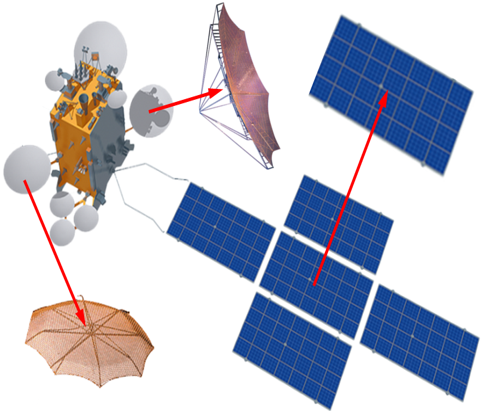
\includegraphics[width = 1\textwidth]{images/synopsis/decomposition}
			\end{column}
			\begin{column}{0.5\textwidth}
				\centering
				% Определение стиля
				\tikzstyle{blockWide}=[rectangle, draw = black, fill = blue!20, rounded corners, text width = 20em, text centered, minimum height = 1.5em, drop shadow] % Блок
				\tikzstyle{blockWideC}=[blockWide, fill = red!20]
				\tikzstyle{arrow} = [draw, thick, color=black!90, -latex'] % Стрелка
				\scriptsize % Размер шрифта
				% Задание перменных
				\def\nodeDist{0.3cm} % Дистанция между узлами
				% Отрисовка блок-схемы
				\begin{tikzpicture}[scale = 1, transform shape]
					% Задание узлов		
					\node (modalTests) [blockWide] {Модальные испытания составных частей конструкции};
					\node (modelUpdating) [blockWide, below = \nodeDist of modalTests] {Коррекция расчетных моделей составных частей конструкции по результатам испытаний};
					\node (checkInfluence) [blockWide, below = \nodeDist of modelUpdating] {Освобождение закрепленных расчетных моделей составных частей конструкции};
					\node (buildRealModel) [blockWide, below = \nodeDist of checkInfluence] {Синтез расчетной модели полной конструкции из её составных частей};
					\node (buildMathModel) [blockWide, below = \nodeDist of buildRealModel] {Определение динамических характеристик полной расчетной модели};
					% Соединение узлов
					\draw [arrow] (modalTests.south) -- (modelUpdating.north);
					\draw [arrow] (modelUpdating.south) -- (checkInfluence.north);
					\draw [arrow] (checkInfluence.south) -- (buildRealModel.north);
					\draw [arrow] (buildRealModel.south) -- (buildMathModel.north);
				\end{tikzpicture}
			\end{column}
		\end{columns}
		\vspace{0.2em}
		Схема методики синтеза глобальных расчетных моделей
	\end{center}
	\vspace{-0.6em}
	\begin{block}{Достоинства методики}
		\begin{itemize}
			\setlength{\itemsep}{0pt}
			\item Составные части обладают более высокими частотами собственных колебаний.
			\item Не требуется больших помещений для проведения испытаний.
			\item Меньшее влияние воздушной среды на определяемые динамические характеристики.
		\end{itemize} 
	\end{block}
\end{frame}

\begin{frame}{Построение матриц демпфирования составных частей}
	\begin{center}
		\begin{columns}
			\begin{column}{0.54\textwidth }
				\centering
				\vspace{-0.75em}
				\includegraphics[width = 1\textwidth]{ms-21}
				Модальные испытания МС-21
			\end{column}
			\begin{column}{0.45\textwidth}
				\centering
				\begin{tikzpicture}[scale = 1]
					\small
					\pgfmathsetmacro{\vertStep}{0.6}
					\begin{axis}[
						xlabel            = {$ \overline{f} $},
						ylabel            = {$ \lambda $}, 
						ylabel shift      = -5 pt,
						width             = 5.7cm,
						grid              = both,
						mark size         = 1pt,
						ylabel near ticks,
						xlabel near ticks,
						xmin = 0.985, xmax = 1.025
					]
						\pgfplotstableread{images/presentation/monophase-parameter.txt}\contentFile
						\addplot table [x index = 0, y index = 1] {\contentFile};
						\addplot table [x index = 0, y index = 2] {\contentFile};
						\node[text width = 25mm] at (axis cs: 1.012, -1.55) {Вертикальный изгиб фюзеляжа};
						\draw[very thick, dashed, color = teal] (axis cs:1, -\vertStep) -- (axis cs:1, \vertStep);
						\node[color = teal] at (axis cs: 0.996, 0.5) {$ \overline{f}_\text{рез} $};
					\end{axis}
				\end{tikzpicture}
			\end{column}
		\end{columns}
	\end{center}
	\vspace{-1em}
	\begin{block}{Нулевое приближение по гипотезе Сорокина}
		\begin{equation}
			\begin{gathered}
			\mat{H} = \alpha \tilde{\mat{K}} + \beta \mat{M}, \\
			G(\alpha, \beta) = \sum\limits_{i\,=\,1}^p w_i \left( 1 - \frac{\alpha \tilde{\kappa}_i + \beta \mu_i}{h_i} \right)^2 \rightarrow \min_{\alpha, \beta}.
			\end{gathered}
		\end{equation}
	\end{block}
	\vspace{-0.5em}
	\begin{block}{Введение корректирующих элементов}
		\begin{equation}
			\tilde{\mat{H}} = \mat{H} + \Delta \internal{\mat{H}} + \Delta \external{\mat{H}}.
		\end{equation}
	\end{block}
\end{frame}

\begin{frame}{Тестирование методики синтеза на примере модели КА}
	\begin{center}
		\begin{tikzpicture}
			\pgfmathsetmacro{\horizDist}{5}
			\pgfmathsetmacro{\vertDist}{0.75}
			\pgfmathsetmacro{\shiftText}{0.01}
			\tikzstyle{arrow} = [draw, line width = 0.5mm, -{Latex[length = 3mm]}, color = blue] 
			% Полная модель
			\node[inner sep = 0pt] (mesh) at (0, 0) {\includegraphics[width = 0.7\textwidth]{images/presentation/spacecraft-test-mesh}};
			\node[inner sep = 0pt, below = \shiftText of mesh.south] (textMesh) {Глобальная модель};
			% Орбитальный модуль
			\draw (mesh.south) ++ (-\horizDist/2, -\vertDist) node [below] (orbital) {\includegraphics[width = 0.35\textwidth]{test-spacecraft-orbital-distribution}};
			\node[inner sep = 0pt, below = \shiftText of orbital.south] (textOrbital) {а) Орбитальный модуль};
			% Панели солнечных батарей
			\draw (mesh.south) ++ (\horizDist/2, -\vertDist) node [below] (panel) {\includegraphics[height = 0.33\textwidth]{test-spacecraft-panel-distribution}};
			\node[inner sep = 0pt, below = \shiftText of panel.south] (textPanel) {б) Панели солнечных батарей};
			% Стрелки
			\draw [arrow] (textMesh.west) ++ (-0.3, 0) -- (orbital.north);
			\draw [arrow] (textMesh.east) ++ (0.3, 0) -- (panel.north);
		\end{tikzpicture}
		
		Изменения узловых жесткостей при коррекции моделей составных частей
	\end{center}	
\end{frame}

\begin{frame}{Результаты синтеза глобальной модели КА}
	\begin{center}
		\begin{columns}
			\begin{column}{0.47\textwidth}
				\centering
				\small
				\begin{tikzpicture}[scale = 1]
					\hspace{-0.5em}
					\begin{semilogyaxis}[
						xlabel            = {Номер итерации коррекции},
						ylabel            = {$ \lVert \mat{\alpha} \rVert_{\max} $}, 
						ylabel shift      = -5 pt,
						width             = 6.25cm,
						grid              = both,
						legend cell align = left,
						legend style      = {
							at            = {(0.02, 0.14)},
							anchor        = west,
							fill          = white,
							fill opacity  = 0.6,
							draw opacity  = 1,
							text opacity  = 1,
						},
						ylabel near ticks,
						xmin = 0, xmax = 8
					]
						\addplot table {images/partModelUpdating/test-spacecraft-panels-convergence.txt};
						\addplot table {images/partModelUpdating/test-spacecraft-orbital-convergence.txt};
						\legend{Панели, Орбитальный модуль}
					\end{semilogyaxis}
				\end{tikzpicture}
				Оценка сходимости коррекции по частотному критерию
			\end{column}
			\hfill
			\begin{column}{0.52\textwidth}		
				\centering
				\begin{tblr}{
					colspec = {|X[c, -1]|X[c]|X[c]|X[c]|X[c]|},
					hlines,
					colsep = 1pt,
					rows = {font = \footnotesize}
				}
					\SetCell[r = 3]{c} Тон & \SetCell[c = 4]{c} Погрешность в частотах, \% &&& \\
					& \SetCell[r = 2]{c} Исходная & \SetCell[c = 3]{c} После коррекции && \\
					& & Панелей & Модуля & {Панелей \\ и модуля} \\ \hline
					7 & -4.689 & -2.120 & -2.756 & -0.021 \\
					8 & -4.678 & -2.078 & -2.782 & -0.018 \\
					9 & -5.121 & -4.447 & -0.674 & 0.100  \\
					10 & -5.040 & -4.760 & -0.354 & -0.028 \\
					11 & -5.040 & -4.760 & -0.357 & -0.032 \\
					12 & -5.121 & -4.443 & -0.687 & 0.091 \\
					13 & -4.102 & -0.966 & -3.161 & 0.011 \\
					14 & -4.112 & -0.999 & -3.135 & 0.016 \\
					15 & -3.303 & -0.234 & -3.066 & -0.006 \\
					16 & -3.303 & -0.234 & -3.066 & -0.005 \\
				\end{tblr}
			\end{column}
		\end{columns}
	\end{center}
\end{frame}

\section{Положения, выносимые на защиту (продолжение)}

\begin{frame}{Положения, выносимые на защиту}
	\begin{enumerate}
		\setcounter{enumi}{2} 
		\item Обоснована методика формирования глобальной матрицы демпфирования конструкций по результатам испытаний их составных частей.
		\item Развита методика испытаний составных частей ЛА для достоверного построения их матриц жесткости.
	\end{enumerate}
\end{frame}

\section{Программы для обработки и представления результатов модальных испытаний}

\begin{frame}{Программы для обработки и представления результатов модальных испытаний}
	\begin{center}
		\begin{tikzpicture}
			\node[inner sep = 0pt] (gencalc) at (0, 0) {\includegraphics[width = 0.6\textwidth]{gencalc-interface}};
			\node[inner sep = 0pt] (analyzer) at (3, -2) {\includegraphics[width = 0.6\textwidth]{analyzer-interface}};
		\end{tikzpicture}
	\end{center}
\end{frame}

\section{Программа для диагностирования дефектов конструкций по результатам испытаний}

\begin{frame}{Программа для диагностирования дефектов конструкций по результатам испытаний}
	Возможное месторасположение дефекта соответствует максимуму параметра искажений портретов колебаний. Типы обнаруживаемых дефектов: зазоры, люфты и трещины. 
	\begin{center}
		\begin{figure}
			\begin{subfigure}[t]{0.53\textwidth}
				\includegraphics[width = 1\textwidth]{express-amu-7}
			\end{subfigure}
			\begin{subfigure}[t]{0.45\textwidth}
				\includegraphics[width = 1\textwidth]{distortion-spacecraft}
			\end{subfigure}
		\end{figure}
		Обнаружение зазоров в узлах установки солнечных батарей
	\end{center}
\end{frame}

\section{Операционный модальный анализ по результатам летных испытаний}

\begin{frame}{Операционный модальный анализ по результатам летных испытаний}

	\begin{center}
		\begin{columns}
			\begin{column}{0.55\textwidth}
				\centering
				\textbf{Методика определения критической скорости флаттера}:
				\begin{itemize}
					\setlength{\itemsep}{0pt}
					\raggedright
					\item выход летательного аппарата на исследуемый скоростной режим;
					\item задание генератором сигналов в систему управления; 
					\item передача системой управления воздействий отклоняемым поверхностям;
					\item регистрация колебаний тензодатчиками и акселерометрами до полного завершения переходных процессов;
					\item обобщение и обработка результатов измерений на различных скоростях полета.
				\end{itemize}
			\end{column}		
			\begin{column}{0.43\textwidth}
				\centering
				\begin{tikzpicture}[scale = 1]
					\hspace{-1em}
					\small
					\begin{axis}[
						xlabel            = {$ v $, км/ч},
						ylabel            = {$ \delta $},
						ylabel shift      = -2 pt,
						y dir             = reverse,
						grid              = major,
						legend columns    = 1,
						legend cell align = {left},
						legend style      = {
							at            = {(0.025, 0.68)},
							anchor        = west,
							fill          = white,
							fill opacity  = 0.6,
							draw opacity  = 1,
							text opacity  = 1,
						},
						ylabel near ticks,
						ymin = 0,
						x tick label style = {
							/pgf/number format/.cd,
							set thousands separator = {},
							fixed
						},
						y tick label style = {
							/pgf/number format/.cd,
							fixed
						},
						ylabel near ticks,  
						try min ticks    = 6,
						mark size        = 1.25pt,
						width            = 5.5cm,
						height           = 5.75cm,
					]
						\pgfplotstableread{images/synopsis/flight-decrements-2.txt}\contentFile
						\addplot[color = blue, thick, mark = *, smooth, tension = 0.2] table [x index = 0, y index = 1] {\contentFile};
						\addplot[color = gray, thick, mark = triangle*, smooth, tension = 0.2] table [x index = 0, y index = 2] {\contentFile};
						\addplot[color = teal, thick, mark = diamond*, smooth, tension = 0.2] table [x index = 0, y index = 3] {\contentFile};
						\addplot[color = red, thick,  mark = halfcircle*, smooth, tension = 0.2] table [x index = 0, y index = 4] {\contentFile};
						\addplot[color = orange, thick, densely dashed, mark = o, mark options = {solid}, smooth, tension = 0.2] table [x index = 0, y index = 5] {\contentFile};
						\addplot[color = violet, thick, densely dashed, mark = o, mark options = {solid}, smooth, tension = 0.2] table [x index = 0, y index = 6] {\contentFile};
						\legend{\name{SSI-DD}, \name{ERA}, \name{ADA}, \name{N4SID}, {\name{ЛИИ}, оценка сверху}, {\name{ЛИИ}, оценка снизу}}
					\end{axis}
				\end{tikzpicture}
				Скоростные зависимости логарифмического декремента Су-30
			\end{column}
		\end{columns}
	\end{center}
\end{frame}

\section{Определение динамических характеристик рефлектора по результатам акустических испытаний}

\begin{frame}{Определение модальных характеристик рефлектора по результатам акустических испытаний}
	\textbf{\underline{Принимаемые гипотезы}}:
	\begin{itemize}
		\item динамическая система является стационарной;
		\item исследуемый объект является наблюдаемым: расположение датчиков на конструкции позволяет однозначно идентифицировать формы колебаний, частоты которых лежат в интересующем диапазоне.
	\end{itemize}
	\begin{center}
		\begin{figure}
			\centering
			\small
			\begin{subfigure}[t]{0.49\textwidth}
				\includegraphics[width = 1\textwidth]{reflector-experiment}
				а) Рефлектор в акустической камере
			\end{subfigure}
			\hfill
			\begin{subfigure}[t]{0.49\textwidth}
				\includegraphics[width = 1\textwidth]{reflector-sensors} 
				б) Расположение датчиков на поверхности рефлектора
			\end{subfigure}
		\end{figure}
		\vspace{0.5em}
		Проведение акустических испытаний
	\end{center}
\end{frame}

\begin{frame}{Результаты определения динамических характеристик рефлектора методами операционного модального анализа}
	\centering
	\vspace{0.5em}
	\begin{tblr}{
		colspec = {|c|c|c|c||c|c|c|},
		hlines,
		rows = {font = \footnotesize}
	}
		\SetCell[r = 2]{c} Тон & \SetCell[c = 3]{c} Частота $ f $, Гц && & \SetCell[c = 3]{c} Логарифмический декремент $ \delta $ && \\
		& SSI-COV & ERA & SSI-DD & SSI-COV & ERA & SSI-DD \\ \hline
		1 & 66.052 & 65.962 & 66.403 & 0.054 & 0.042 & 0.045 \\
		2 & 91.287 & 90.910 & 91.843 & 0.030 & 0.052 & 0.042 \\
		3 & 102.540 & --- & --- & 0.056 & --- & --- \\
		4 & 114.770 & --- & --- & 0.063 & --- & --- \\
		5 & 122.370 & --- & --- & 0.094 & --- & --- \\
	\end{tblr}
	\begin{columns}
		\footnotesize
		\begin{column}{0.25\textwidth}
			\centering
			\includegraphics[width = 1\textwidth]{reflector-ssi-cov-mode-1}
			$ f = 91.29 $ Гц, $ \delta = 0.03 $ 
		\end{column}
		\begin{column}{0.25\textwidth}	
			\centering
			\includegraphics[width = 1\textwidth]{reflector-ssi-cov-mode-2} 
			$ f = 127.85 $ Гц, $ \delta = 0.05 $
		\end{column}
		\begin{column}{0.25\textwidth}	
			\centering
			\includegraphics[width = 1\textwidth]{reflector-ssi-cov-mode-4} 
			$ f = 325.36 $ Гц, $ \delta = 0.03 $
		\end{column}
	\end{columns}
	\vspace{0.5em}
	Идентифицированные тона колебаний
\end{frame}

\section{Решение практических задач коррекции расчетных моделей}

\section{Коррекция расчетной модели динамически-подобной модели самолета Ту-204}

\begin{frame}{Коррекция расчетной модели динамически-подобной модели самолета Ту-204}
	Геометрические и физические характеристики модели:
	\begin{columns}
		\begin{column}{0.45\textwidth}
			\begin{itemize}
				\item Размах крыла --- $ 3172 $ мм.
				\item Длина фюзеляжа --- $ 3462 $ мм.
			\end{itemize}
		\end{column}
		\begin{column}{0.55\textwidth}
			\begin{itemize}
				\item Масштаб моделирования --- $ 1 \div 10 $.
				\item Масса модели --- $ 50.5 $ кг.
			\end{itemize}
		\end{column}
	\end{columns}
	\begin{center}
		\begin{figure}
			\small
			\begin{subfigure}[t]{0.49\textwidth}
				\centering
		     	\includegraphics[width = 1\textwidth]{tu-204-experiment} 
		     	а) Упругое вывешивание модели
		    \end{subfigure}
	    	\hfill
		    \begin{subfigure}[t]{0.49\textwidth}
				\centering
				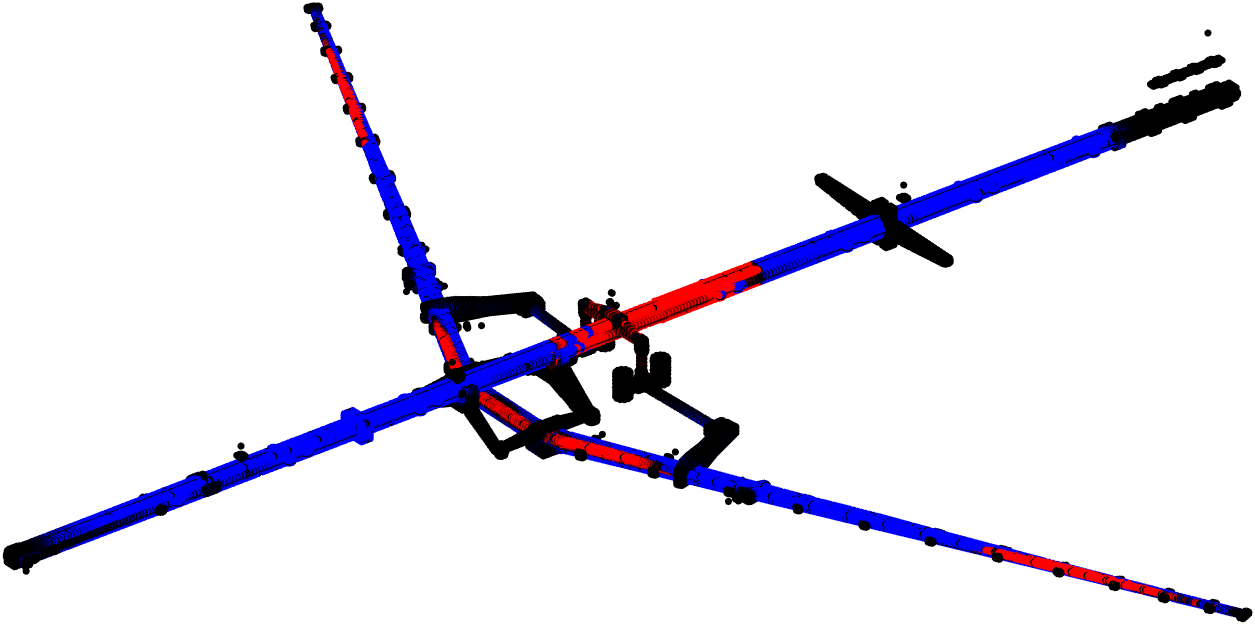
\includegraphics[width = 1\textwidth]{tu-204-coeffs-6}
				б) Изменение узловых жесткостей
		    \end{subfigure}
		\end{figure}
		\vspace{1em}
		Динамически-подобная модель самолета Ту-204
	\end{center}
\end{frame}

\begin{frame}{Результаты применения методики коррекции} 
	\resizebox{\textwidth}{!}{%
	\begin{tblr}
	{
		colspec = {|c|c|c|c|c|c|c|c|c|c|}, 
		hlines
	}
   		\SetCell[r = 3]{c} Тон & \SetCell[c = 2]{c} Частоты, Гц && \SetCell[c = 7]{c} Погрешность до и после коррекции, \%  \\
	   	& \SetCell[r = 2]{c} Эксперимент & \SetCell[r = 2]{c} {Исходная \\ модель} & \SetCell[r = 2]{c} До & \SetCell[c = 6]{c} После \\ 
   		& & & & 1 & 2 & 3 & 4 & 5 & 6 \\ \hline
		СИКр1\footnotemark[1] & 3.44 & 3.49 & 1.5 & 0.0 & 0.0 & 0.0 & 0.0 & 0.0 & 0.0 \\
		АСИКр1\footnotemark[2] & 4.87 & 4.96 & 1.7 & -0.6 & 0.0 & 0.0 & 0.0 & 0.0 & 0.0 \\
		ГИФ1\footnotemark[3] & 5.44 & 5.73 & 5.3 & 4.7 & 4.7 & 0.0 & 0.0 & 0.0 & 0.0 \\ 
		ВИФ1\footnotemark[4] & 5.73 & 5.97 & 4.2 & 3.5 & 3.3 & 2.6 & 0.0 & 0.0 & 0.0 \\
		СИКр2\footnotemark[5] & 9.30 & 9.13 & -1.8 & -4.4 & -3.2 & -3.9 & -4.4 & 0.0 & 0.0 \\
		ВИФ2\footnotemark[6] & 14.18 & 14.77 & 4.2 & 3.7 & 3.8 & 3.4 & 2.0 & 3.3 & 0.0 \\
	\end{tblr} }
	\footnotetext[1]{Cимметричный изгиб крыла I тона}
	\footnotetext[2]{Антисимметричный изгиб крыла I тона}
	\footnotetext[3]{Горизонтальный изгиб фюзеляжа I тона}
	\footnotetext[4]{Вертикальный изгиб фюзеляжа I тона}
	\footnotetext[5]{Симметричный изгиб крыла II тона}
	\footnotetext[6]{Вертикальный изгиб фюзеляжа II тона}
\end{frame}

\section{Синтез имитационной модели каркаса зонтичной антенны космического аппарата}

\begin{frame}{Синтез имитационной модели каркаса зонтичной антенны космического аппарата}
	\begin{center}
		\begin{tikzpicture}
			\small
			\pgfmathsetmacro{\vertDist}{4}
			\pgfmathsetmacro{\shiftText}{0.05}
			\tikzstyle{arrow} = [draw, line width = 0.5mm, -{Latex[length = 2.5mm]}, color = blue] 
			% Полная модель
			\node (boundary) at (0, 0) {};
			\draw (boundary.east) ++ (3.25, 0) node (assembly) {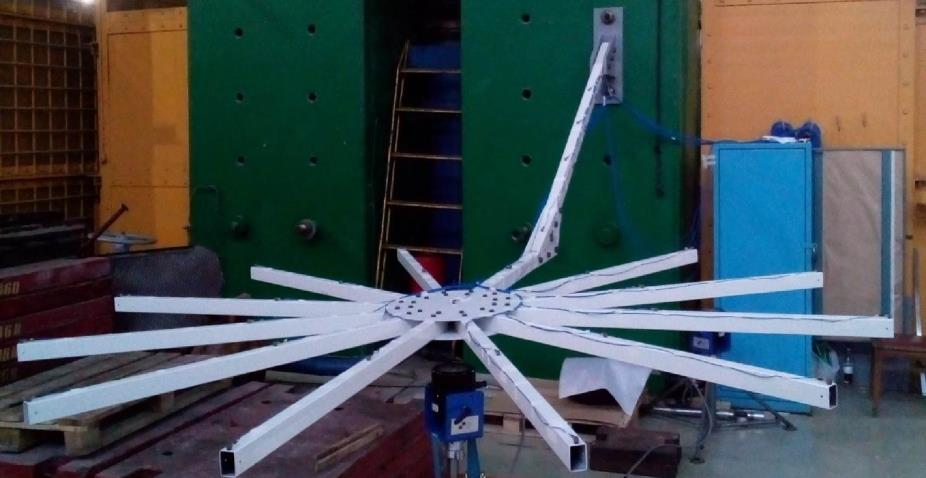
\includegraphics[width = 0.5\textwidth]{simsat-assembly}};
			\node[inner sep = 0pt, below = \shiftText of assembly.south] (textAssembly) {Конструкция в сборе};
			% Сведения
			\draw (assembly.east) ++ (5.75, 0) node (info){
				\vbox				
				{\begin{itemize}
					\item Длина штанги --- $ 2250 $ мм.
					\item Масса штанги --- 22 кг.
					\item Диаметр рефлектора --- $ 3000 $ мм.
					\item Масса рефлектора --- $ 73 $ кг.
				\end{itemize}}
			};
			% Зонтичный каркас
			\node (antenna) at (3, -\vertDist)  {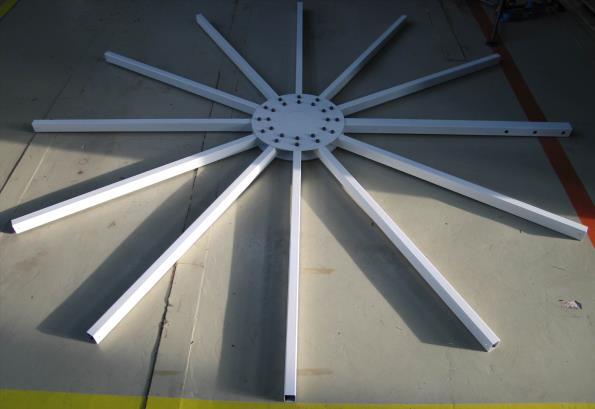
\includegraphics[width = 0.35\textwidth]{simsat-antenna}};
			\node[inner sep = 0pt, below = \shiftText of antenna.south] (textAntenna) {а) Рефлектор};
			% Штанга
			\node (handle) at (8, -\vertDist) {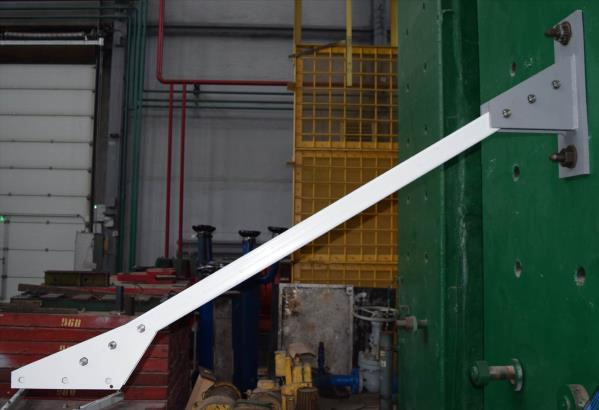
\includegraphics[width = 0.35\textwidth]{simsat-handle}};
			\node[inner sep = 0pt, below = \shiftText of handle.south] (textHandle) {б) Штанга};
			% Стрелки
			\draw [arrow] (antenna.north) ++ (0, 0.45) -- (antenna.north);
			\draw [arrow] (textAssembly.east) ++ (0.2, 0) -- (handle.north);
		\end{tikzpicture}
		
		Имитационная модель каркаса зонтичной антенны
	\end{center}
\end{frame}

\begin{frame}{Результаты применения методики синтеза} 
	\small
	\begin{center}
		\begin{columns}
			\begin{column}{0.6\textwidth}
				\centering
				\includegraphics[width = 1\textwidth]{scheme-fixture}
			\end{column}
			\begin{column}{0.4\textwidth}
				\centering
				\includegraphics[width = 0.7\textwidth]{scheme-springs}
			\end{column}
		\end{columns}
		Расчетные схемы для оценки податливости закреплений в эксперименте \\
		\vspace{0.5em}
		\begin{tblr}
		{
			colspec = {|c|c|c|c|}, 
			hlines,
			colsep = 2pt,
			rows = {font = \footnotesize}
		}
			\SetCell[r = 2]{c} Тон & \SetCell[c = 3]{c} {Погрешность до и после коррекции, \%} \\
			& Исходная & {Коррекция \\ (настоящая методика)} & {Коррекция \\ (Маринин, 2020)} \\ \hline
			1 & 1.84 & 0.70 & 0.66 \\ 
		    2 & 3.88 & 0.40 & 2.76 \\ 
		    3 & 3.19 & 1.24 & 2.97 \\ 
	    	4 & 2.13 & 1.18 & 1.78 \\ 
		    5 & 2.25 & 1.95 & 1.95 \\ 
		\end{tblr}
	\end{center}	
\end{frame}

\section{Коррекция расчетной модели отъемной части крыла изделия С-70}

\begin{frame}{Коррекция расчетной модели отъемной части крыла изделия С-70}
	\begin{center}
		\begin{figure}
			\small
			\begin{subfigure}[t]{0.35\textwidth}
				\centering
		     	\includegraphics[width = 0.7\textwidth]{images/presentation/wing-experiment} \\
		     	Консоль крыла на подвеске
		    \end{subfigure}
		    \begin{subfigure}[t]{0.45\textwidth}
				\centering
				\includegraphics[width = 1\textwidth]{wing-coeffs-5} \\
				Изменение узловых жесткостей
		    \end{subfigure}
		\end{figure}
		\vspace{0.5em}
		\begin{tblr}{
			colspec = {|c|c|c|c|c|c|c|c|c|}, 
			width = \textwidth, 
			hlines,
			rows = {font = \footnotesize}
		}
			\SetCell[r = 3]{c} Тон & \SetCell[c = 2]{c} Приведенная частота && \SetCell[c = 6]{c} Погрешность до и после коррекции, \% \\
			& \SetCell[r = 2]{c} Эксперимент & \SetCell[r = 2]{c} {Исходная \\ модель} & \SetCell[r = 2]{c} До & \SetCell[c = 5]{c}После \\
			& & & & 1 & 2 & 3 & 4 & 5 \\ \hline
			1 & 1.00 & 1.51 & 50.7 & 0.0 & 0.0 & 0.0 & 0.0 & 0.0 \\ 
			2 & 2.28 & 3.18 & 39.5 & -7.4 & 0.0 & 0.0 & 0.0 & 0.0 \\ 
			3 & 3.37 & 4.13 & 22.6 & -18.6 & -13.8 & 0.0 & 0.0 & 0.0 \\ 
			4 & 3.95 & 4.82 & 21.8 & -19.1 & -17.8 & -8.2 & 0.0 & 0.0 \\ 
			5 & 4.87 & 6.15 & 26.2 & -16.2 & -21.8 & -2.6 & -4.4 & 0.0 \\ 
		\end{tblr}
	\end{center}
\end{frame}

\begin{frame}{Сопоставление форм колебаний до и после коррекции}
	\begin{block}{Критерий модального соответствия (MAC-критерий)}
		\begin{equation}
			\mathrm{MAC}_{i, j} = \frac{(\mat{u}_i ^ \intercal \cdot \mat{v}_j) ^ 2}{(\mat{u}_i ^ \intercal \cdot \mat{u}_i) (\mat{v}_j ^ \intercal \cdot \mat{v}_j)}, 
		\end{equation}
		где $ \mat{u}_i $ и $ \mat{v}_j $~---~формы колебаний до и после коррекции; $ i, j = 1 \hdots n $.
	\end{block}
	\vspace{-0.5em}
	\begin{columns}
		\begin{column}{0.49\textwidth}
			\centering
			\begin{figure}
				\includegraphics[width=1\textwidth]{wing-MAC}
			\end{figure}
		\end{column}
		\begin{column}{0.4\textwidth}
			\centering
			\begin{figure}
				\includegraphics[width=1\textwidth]{wing-initial-mode-1} \\ \vspace{0.2em}
				\includegraphics[width=1\textwidth]{wing-initial-mode-2} \\ \vspace{0.2em}
				\includegraphics[width=1\textwidth]{wing-initial-mode-3} \\ \vspace{0.2em}
				\includegraphics[width=1\textwidth]{wing-initial-mode-4}
			\end{figure}
		\end{column}
	\end{columns}
\end{frame}

\section{Коррекция расчетной модели гирдера для модульных секций накопителя ЦКП <<СКИФ>>}

\begin{frame}{Коррекция расчетной модели гирдера для модульных секций накопителя ЦКП <<СКИФ>>}
	\vfill
	\begin{center}
		\begin{figure}
			\small
			\begin{subfigure}[b]{0.49\textwidth}
				\centering
		     	\includegraphics[width = 1\textwidth]{girder-full-system} 
		     	а) Совместная геометрическая модель гирдера и магнитов
		    \end{subfigure}
	    	\hfill
		    \begin{subfigure}[b]{0.49\textwidth}
				\centering
				\includegraphics[width = 1\textwidth]{girder-experiment}
				б) Модальные испытания гирдера без магнитов
		    \end{subfigure}
		\end{figure}
		\vspace{0.5em}
    	Гирдер для модульных секций накопителя
    \end{center}
\end{frame}

\begin{frame}{Результаты коррекции расчетной модели гирдера}
	\textbf{\underline{Последовательность коррекции}}
	\begin{enumerate}
		\item Уточнение упругих характеристик основания ($ 2 $ минуты).
		\item Коррекция четырех упругих горизонтальных тонов ($ 7 $ минут).
		\item Коррекция двух упругих вертикальных тонов ($ 1 $ минута).
		\item Коррекция всех шести упругих тонов ($ 4 $ минуты).
	\end{enumerate}
	\vfill
	\centering
	\begin{tblr}{
		colspec = {|X[c, -1]|X[c]|X[c]|X[c]|X[c]|}, 
		width = \textwidth, 
		hlines
	}
		\SetCell[r = 2]{c} Тон & \SetCell[c = 2]{c} Частота, Гц && \SetCell[c = 2]{c} Погрешность, \% \\
		& Эксперимент & Исходная модель & До коррекции & После коррекции \\ \hline
		6 & 119.51 & 135.08 & 13.03 & \SetCell[r = 6]{c} \textbf{0.00} \\
		7 & 140.97 & 146.46 & 3.89 &  \\
		8 & 148.13 & 160.07 & 8.06 &  \\
		9 & 189.65 & 210.48 & 10.98 & \\
		10 & 197.53 & 214.18 & 8.43 & \\
		11 & 242.24 & 253.51 & 4.65 & \\
	\end{tblr}
\end{frame}

\section{Свидетельства о регистрации программ и патент на изобретение}

\begin{frame}{Свидетельства о регистрации программ и патент на изобретение}
	\begin{center}
		\begin{columns}
			\begin{column}{0.24\textwidth}
				\centering
				\includegraphics[width = 1\textwidth]{images/presentation/certificate-flightLab} \\ \vspace{0.5em}
				\includegraphics[width = 1\textwidth]{images/presentation/certificate-genCalc}
			\end{column}
			\begin{column}{0.24\textwidth}
				\centering
				\includegraphics[width = 1\textwidth]{images/presentation/certificate-responseAnalyzer} \\ \vspace{0.5em}
				\includegraphics[width = 1\textwidth]{images/presentation/certificate-distortionFinder}
			\end{column}
			\begin{column}{0.3\textwidth}
				\centering
				\includegraphics[width = 1\textwidth]{images/presentation/patent-freeing-front}
			\end{column}
		\end{columns}
	\end{center}
\end{frame}

\section{Акты об использовании и внедрении}

\begin{frame}{Акты об использовании и внедрении}
	\begin{center}
		\begin{columns}
			\begin{column}{0.34\textwidth}
				\centering
				\includegraphics[width = 1\textwidth]{images/presentation/act-oak}
				\textbf{<<ОКБ Сухого>>} \\ (Cy-57, C-70)
			\end{column}
			\begin{column}{0.34\textwidth}
				\centering
				\includegraphics[width = 1\textwidth]{images/presentation/act-skif}
				\textbf{ЦКП <<СКИФ>>} \\ (гирдер)
			\end{column}
			\begin{column}{0.34\textwidth}
				\centering
				\vspace{2.5em}
				\includegraphics[width = 1\textwidth]{images/presentation/act-sibnia}
				\textbf{ФАУ <<СибНИА им.\,С.А.\,Чаплыгина>>} (Су-30, Су-34, Як-130, Як-152, МС-21)
			\end{column}
		\end{columns}
	\end{center}	
\end{frame}

	
	% Заключение	
	%
\section{Научная новизна}

\begin{frame}{Научная новизна}
	\begin{enumerate}
		\item Разработана новая методика коррекции конечно-элементных моделей ЛА, заключающаяся в добавлении корректирующих конечных элементов, параметры которых определяются по результатам модальных испытаний.
		\item Создан способ определения частот и форм собственных колебаний свободной конструкции по результатам испытаний этой конструкции с наложенными связями.
		\item Обоснована методика формирования глобальной матрицы демпфирования конструкций по результатам испытаний их составных частей.
		\item Развита методика испытаний составных частей ЛА для достоверного построения их матриц жесткости.
	\end{enumerate}
\end{frame}

\section{Заключение}

\begin{frame}{Заключение}
	\begin{enumerate}
		\item Разработана методика коррекции конечно-элементных моделей летательных аппаратов по результатам модальных испытаний, основанная на дополнении исходной модели корректирующими конечными элементами.
		\item Исследования сходимости алгоритма и чувствительности методики коррекции расчетных моделей показали, что результаты коррекции устойчивы к погрешностям эксперимента. 
		\item Разработан способ определения собственных частот и форм колебаний свободной конструкции по результатам испытаний этой конструкции с наложенными связями.
		\item Развита методика расчетно-экспериментального модального анализа конструкций по результатам испытаний их составных частей. Разработана программа и обоснованы граничные условия в испытаниях составных частей. Создано программное обеспечение, реализующее полный цикл операций для решения задачи синтеза глобальных расчетных моделей из скорректированных моделей составных частей.
	\end{enumerate}
\end{frame}

\begin{frame}{Заключение}
	\begin{enumerate}
		\setcounter{enumi}{4}
		\item Формирование глобальной матрицы демпфирования конструкций по результатам испытаний их составных частей осуществляется в несколько этапов: по соотношениям между вынужденными монофазными и собственными колебаниями подтверждается диагональный вид матриц демпфирования составных частей в главных координатах, определяются обобщенные характеристики демпфирования. На основании гипотезы Е.\,С.~Сорокина строятся начальные приближения матриц демпфирования составных частей в физической системе координат. Эти матрицы уточняются решением задачи коррекции. Формирование глобальной матрицы осуществляется посредством ассемблирования матриц демпфирования составных частей. 
		\item С целью получения исходных данных для коррекции создан комплекс программ, позволяющий проводить обработку и представление результатов модального анализа непосредственно в процессе испытаний. Разработано программное обеспечение для контроля параметров технического состояния изделий в процессе испытаний.
		\item Эффективность разработанных методик и программного обеспечения подтверждена результатами решения практических задач коррекции расчетных моделей конструкций.
	\end{enumerate}
\end{frame} 
	
	% Приложение
	%\appendix
	%
\begin{frame}{Приложение. Акт готовности Як-152 к частотным испытаниям}
	\centering
	\begin{figure}
		\includegraphics[width = 0.65\textwidth]{act-mass}
	\end{figure}
\end{frame}
\end{document}